\documentclass{article}

% Language setting
% Replace `english' with e.g. `spanish' to change the document language
\usepackage[french]{babel}
\usepackage[fleqn]{amsmath} % Aligner les équations à gauche


% Set page size and margins
% Replace `letterpaper' with`a4paper' for UK/EU standard size
\usepackage[letterpaper,top=2cm,bottom=2cm,left=3cm,right=3cm,marginparwidth=1.75cm]{geometry}

% Useful packages
\usepackage{amsmath}
\usepackage{graphicx}
\usepackage{subcaption}
\usepackage[colorlinks=true, allcolors=blue]{hyperref}

\title{TD4}
\author{IPESUP - PC }
\date{11 Décembre 2024}

\begin{document}
\maketitle



\section{Rappels de cours}
Loi de Fourier: 
\\[0.1cm]

$\vec{j}=-\lambda \vec{grad} (T) $
\\[0.1cm]

Résistance thermique : \\
Soit un volume $V$, parallélépipèdique, de surface $S$ et de longueur $l$, de normale $\vec{n}$. On définit le flux thermique surfacique $\Phi$ par la relation : $\Phi = \int_S \vec{j}.\vec{n} dS$. \\
La résistance thermique $R_{th}$ est définie par la relation : $\Phi = \frac{\Delta T}{R_{th}}$, avec $\Delta T$ la différence de température entre les deux faces de la surface $S$.
On a $R_{th} = \frac{L}{\lambda S}$, avec $L$ la longueur de la surface $S$ et $\lambda$ la conductivité thermique du matériau.

Equation de diffusion thermique avec terme de source:
\\[0.1cm]

$\rho c \frac{\partial T}{\partial t }=\lambda \Delta (T) + \mathcal{P}_v$ 
\\[0.2cm]
Coefficient de diffusivité thermique: 
\\[0.1cm]

$a=\frac{\lambda}{\rho c}$
 \\[0.1cm]

Résistance thermique: 
\\[0.1cm]

$R_{th} = \frac{L}{\lambda S}$


\begin{figure}[h]
  \centering
  \begin{subfigure}{0.3\textwidth}
    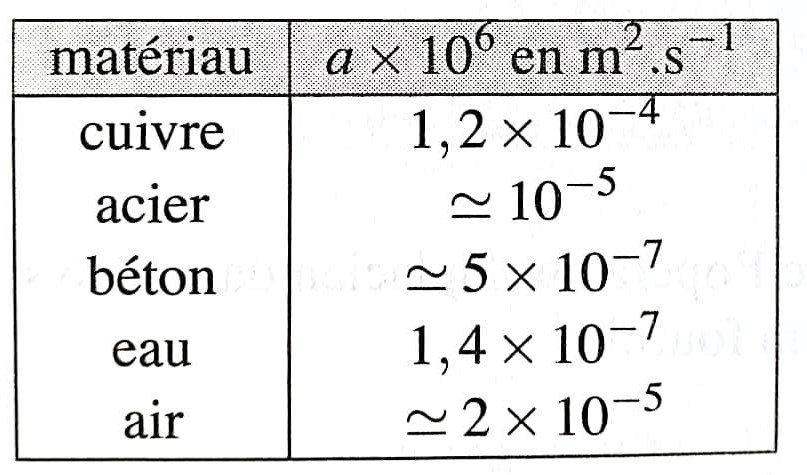
\includegraphics[width=\linewidth]{cs1.jpg}
    \caption{Quelques valeurs de diffusivité thermique}
    \label{fig:subfig1}
  \end{subfigure}
  \hfill
  \begin{subfigure}{0.4\textwidth}
    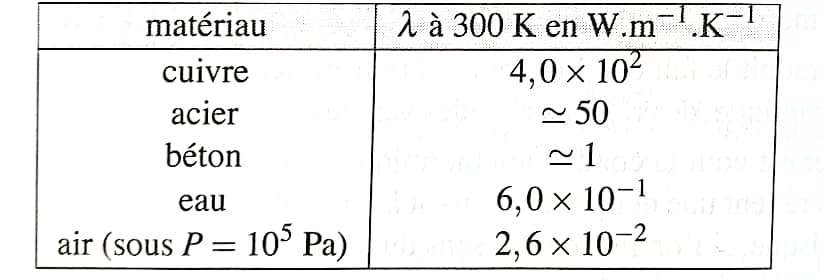
\includegraphics[width=\linewidth]{cs2.jpg}
    \caption{Quelques valeurs de conductivité thermique}
    \label{fig:subfig2}
  \end{subfigure}
  \caption{Valeurs utiles}
  \label{fig:general}
\end{figure}
 
\textbf{Capacités exigibles : }\\

\begin{enumerate}
  \item Enoncer la loi de Fourier
  \item Faire un premier principe local et en déduire la loi de diffusion thermique
  \item Notion de résistance thermique. 
  \item Coefficient de Newton, transferts conducto convectifs.  
\end{enumerate}

\section{Les pingouins}
On modélise un pingouin par un parallépipède rectangle de section carrée de côté $a=10cm$ et de hauteur $l = 50 cm$  Le pingouin maintient sa température interne $T = 37 $°$ C$ au moyen
d'un apport métabolique $\mathcal{P}_1 = 50 W $ qui compense les pertes par conduction thermique au
travers de son revêtement de plumes d'épaisseur $e = 1,0 $ $cm$ et de conductivité thermique $\lambda$.



\begin{figure}[h]
  \centering
  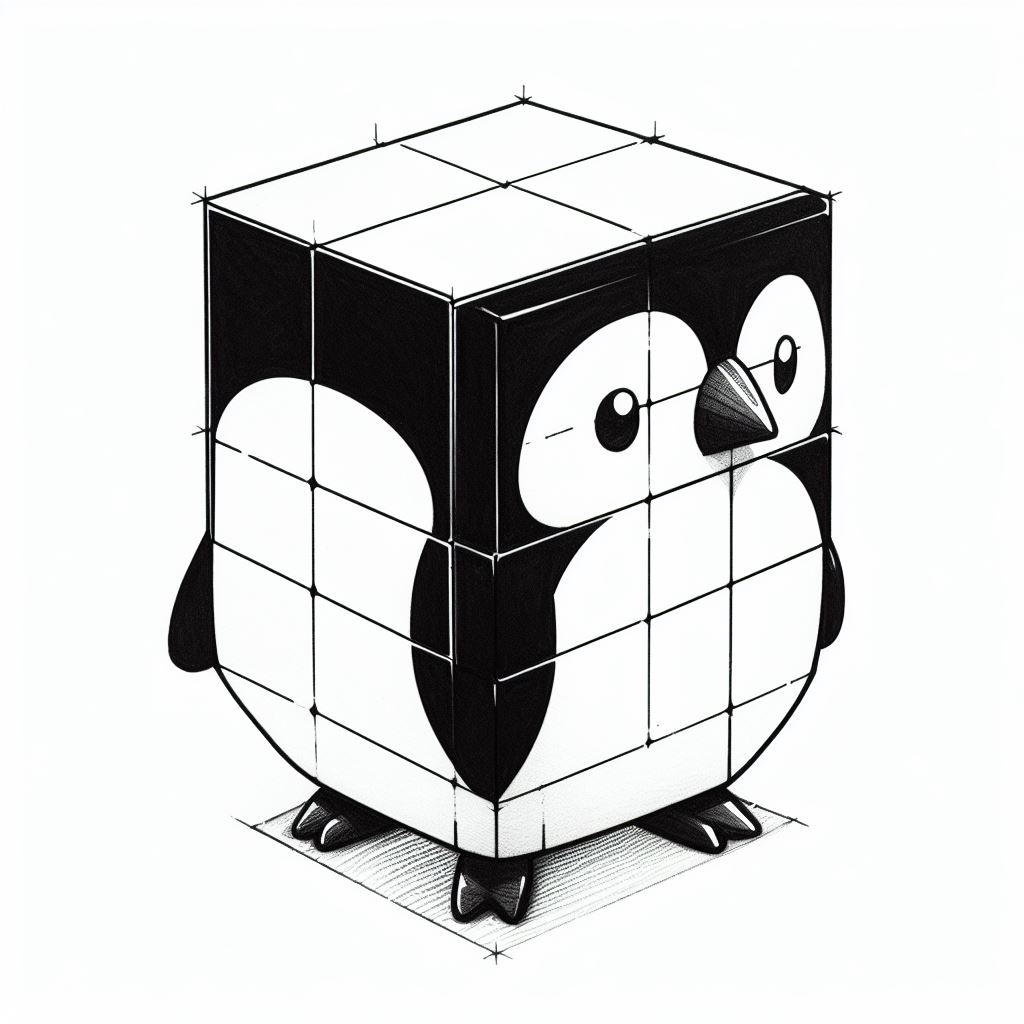
\includegraphics[width=0.4\textwidth]{pingouin_schema.jpeg}
  \label{fig:maison}
    \caption{Schéma d'un pingouin parallélépipèdique}


\end{figure}
\begin{enumerate}
    \item Déterminer la valeur de la conductivité thermique $\lambda $ du revêtement de plume sachant que
la température extérieure (y compris au niveau du sol) est $T_e = -20$°$C$.
\item Pour faire face à des températures extrêmes, neuf pingouins se serrent les uns contre les
autres, formant un carré de 3 x 3 pingouins. Le pavage est parfait, seules les faces supérieures,
inférieures et latérales périphériques sont sujettes aux pertes thermiques.
De combien le métabolisme nécessaire au maintien de la température interne, rapporté à un
pingouins, est-il réduit lorsque les neuf pingouins se serrent les uns contre les autres ?


\section{Puits Canadien} Le puits canadien est un système de préchauffage passif de l’air utilisant les réserves d’énergie
du sol entourant la maison. En faisant passer l’air dans une canalisation enterrée dans le
sol, celui-ci se réchauffe, ce qui permet de réduire fortement la consommation électrique de
chauffage en hiver, ainsi que les émissions de $CO_2$, qui en résultent. Dans cet exercice, un
modèle simple de ce dispositif est étudié.
Une entrée d'air est située à une distance $L$ de la maison. Une pompe à l’intérieur de la maison
permet de faire circuler l’air dans un tuyau de section $ S$ enterré à une profondeur $h$ dans le
sol. 



\begin{figure}[h]
  \centering
  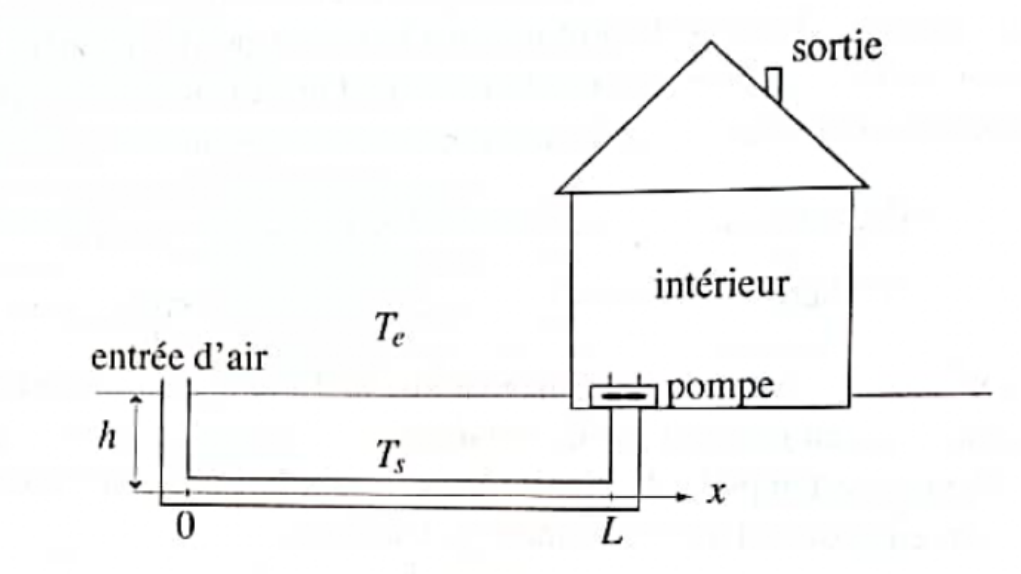
\includegraphics[width=0.4\textwidth]{maison.png}
  \label{fig:maison}
    \caption{Schéma de fonctionnement d'un puits canadien}


\end{figure}


On suppose que les échanges thermiques ne se font que dans la partie horizontale de la canalisation (cylindre de rayon $ R$), comprise entre les abscisses $ x = 0$ et $ x = L$. L’air est considéré comme un gaz parfait de capacité thermique massique à pression constante $c_p$, de masse volumique $\mu$ et de conductivité thermique $\lambda$. On suppose que la température $ T (x)$ est uniforme sur une section droite du tube. L'air se déplace à la vitesse $ v $ constante et uniforme. il entre dans la canalisation  en $ x = O$, à la température $T_e = 10$ °C.

Les échanges thermiques le long de la paroi entre l’air et le sol sont décrits par le flux thermique surfacique : $\Phi = h(T(x)-T_s)$, où $h=$ 6,5 $W.m^{-2}.K^{-1}$
\begin{enumerate}
    \item En supposant que la température extérieure suit la loi $T(0,t) = T_e + T_1 cos(\omega t)$, déterminer la loi de variation de la température dans le sol $T(z,t)$ en la cherchant de la forme $T(z,t) = T_0 + f(z)cos(\omega t - \phi(z))$, avec z la profondeur, nulle à la surface. A quelle profondeur doit-on enterrer la canalisation pour que les variations de température du sol autour de cette dernière soient inférieures à 2°$C$ ? 
    \\
    Dans la suite, on considérera  que la température du sol autour de la canalisation est uniforme et constante et vaut $T_s$
    \item En appliquante le premier principe de la thermodynamique au système fermé constitué de l'air contenu dans la portion de canalisation comprise entre les plans d'abscisse $x$ et $x+dx$ à l'instant $t$, montrer que la température $T(x)$ vérifie l'équation : 
    \begin{equation}
        \frac{d^2T}{dx^2} - \frac{c_p \mu v}{\lambda} \frac{dT}{dx} - \frac{2h}{\lambda R} (T(x)-T_s)=0
    \end{equation}
    \item À quelle condition sur $\lambda$,$L$,$\mu$, $c_p$ et $v$ peut-on  négliger le transfert thermique par diffusion devant le transfert thermique par convection  ? Donner un ordre de grandeur de la vitesse de l'air dans le tuyau pour que cette approximation soit valable. Simplifier alors $(1)$
    \item Résoudre cette équation en faisant apparaitre une longueur caractéristique $\delta$ à exprimer en
fonction des paramètres du problème. 
\item  Établir l’expression littérale de la longueur $L $ de canalisation nécessaire à l’obtention d’une
température d’entrée de l’air dans la maison égale à $T_L$ donnée. Pourquoi le puits permet de
réduire fortement la consommation électrique de chauffage ? Quelle peut être l’utilité du puits
en été (il est appelé également « puits provençal ») ? 
\item  Le volume de la maison est $V = 800 m^3$ , le rayon de la canalisation est $R = 10 cm$, l'air
extérieur est à la température $T_e = 30$°$C$. On veut renouveler l’air de la maison en 2 heures.
Quelle doit être la valeur de la vitesse $ v$ ? 
\item Quelle doit être la longueur de la canalisation pour que la température d’entrée de l’air
dans la maison soit de $20$°$C $ ? \\[1cm]
\end{enumerate}

\end{enumerate}


\begin{figure}[h]
  \centering
  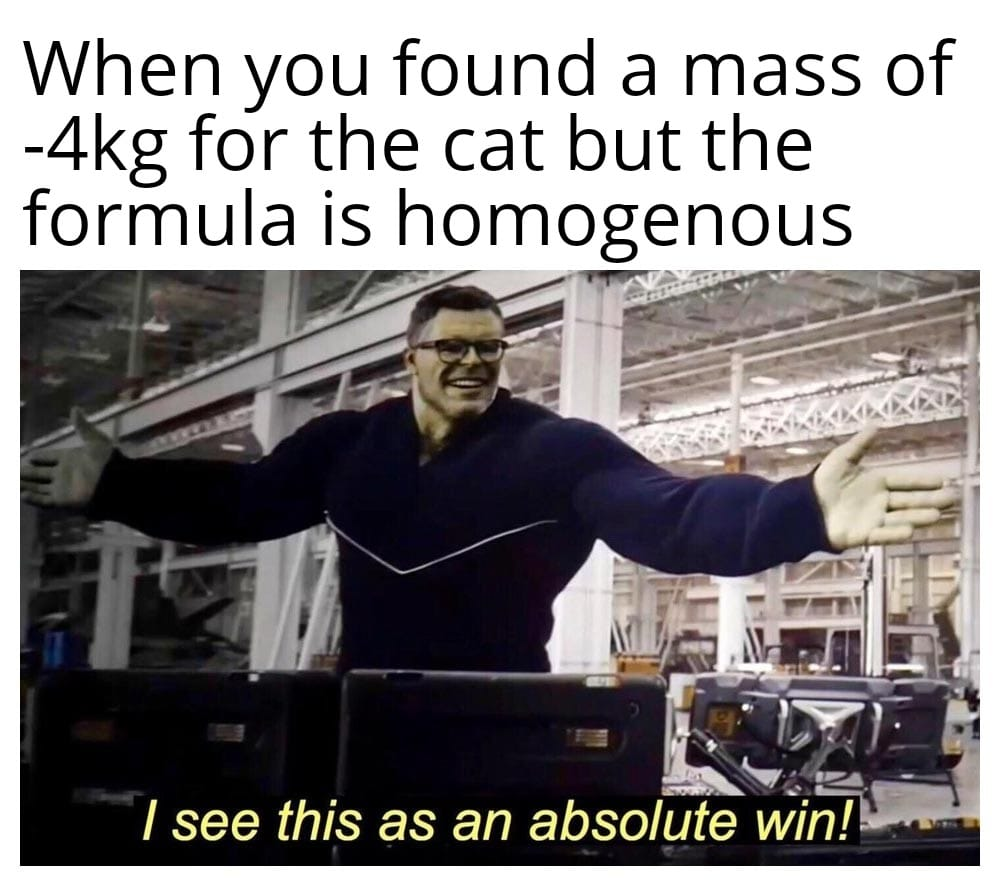
\includegraphics[width=0.4\textwidth]{meme.jpg}
\end{figure}


\end{document}

